\chapter{Конструкторская часть}

В данном разделе будут рассмотрены основные требования к программному обеспечению и схемы алгоритмов.

\section{Требования к программному обеспечению}

Программа должна предоставлять следующие возможности:
\begin{itemize}[left=\parindent]
    \item возможность ввода строки и подстроки;
    \item вывод результата поиска подстроки в строке.
\end{itemize}

\section{Разработка алгоритмов}

На рисунке \ref{img:stand} представлена схема стандартного алгоритма поиска подстроки в строке. На рисунках \ref{img:bm1} -- \ref{img:bm4} показаны
схемы алгоритма Бойера-Мура и дополнительных функций необходимых для поиска подстроки в строке.

\begin{figure}[h]
    \centering
    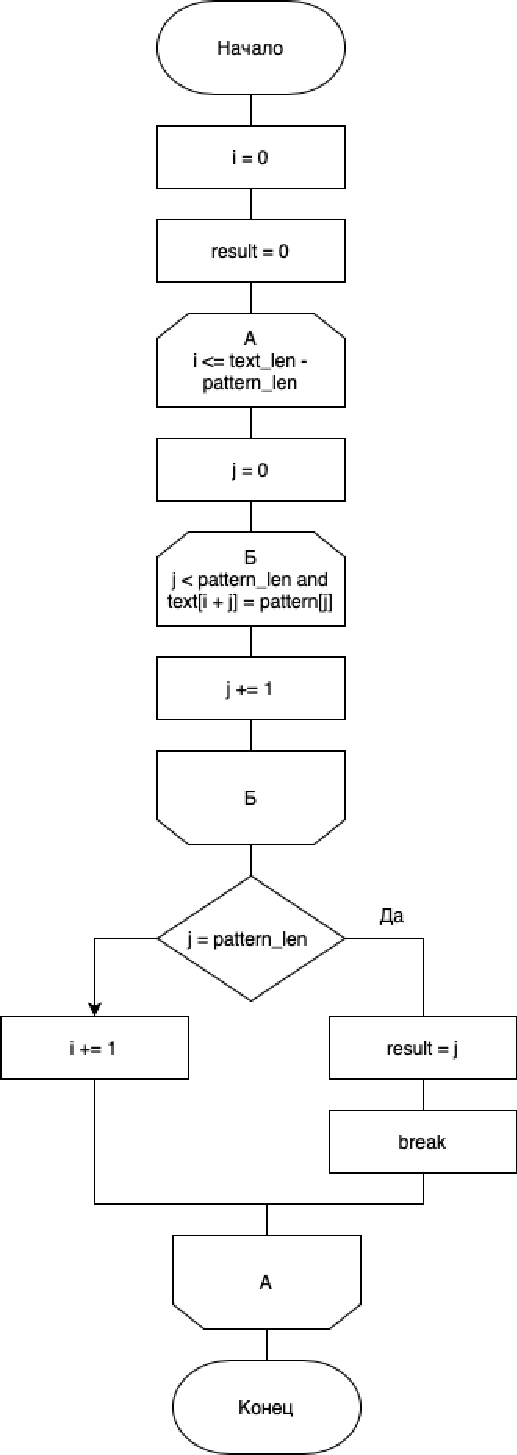
\includegraphics[width=0.5\linewidth]{img/stand.pdf}
    \caption{Схема стандартного алгоритма поиска подстроки в строке}
    \label{img:stand}
\end{figure}

\begin{figure}[h]
    \centering
    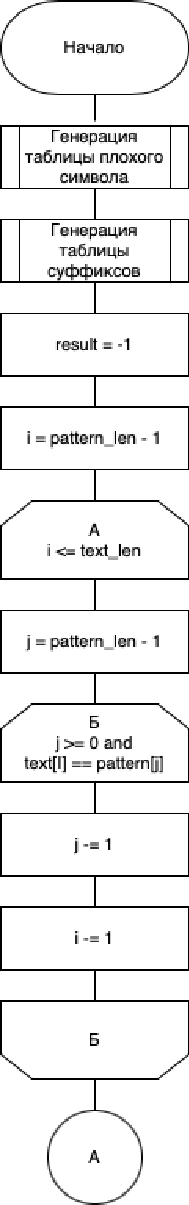
\includegraphics[width=0.2\linewidth]{img/bm1.pdf}
    \caption{Схема алгоритма Бойера-Мура}
    \label{img:bm1}
\end{figure}

\begin{figure}[h]
    \centering
    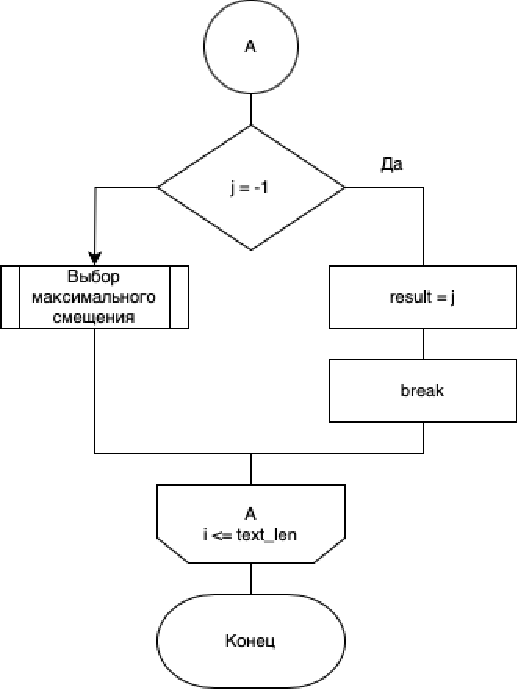
\includegraphics[width=0.5\linewidth]{img/bm2.pdf}
    \caption{Схема алгоритма Бойера-Мура}
    \label{img:bm2}
\end{figure}

\begin{figure}[h]
    \centering
    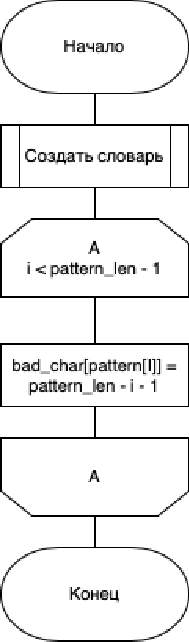
\includegraphics[width=0.2\linewidth]{img/bm3.pdf}
    \caption{Схема создания таблицы плохого символа}
    \label{img:bm3}
\end{figure}

\begin{figure}[h]
    \centering
    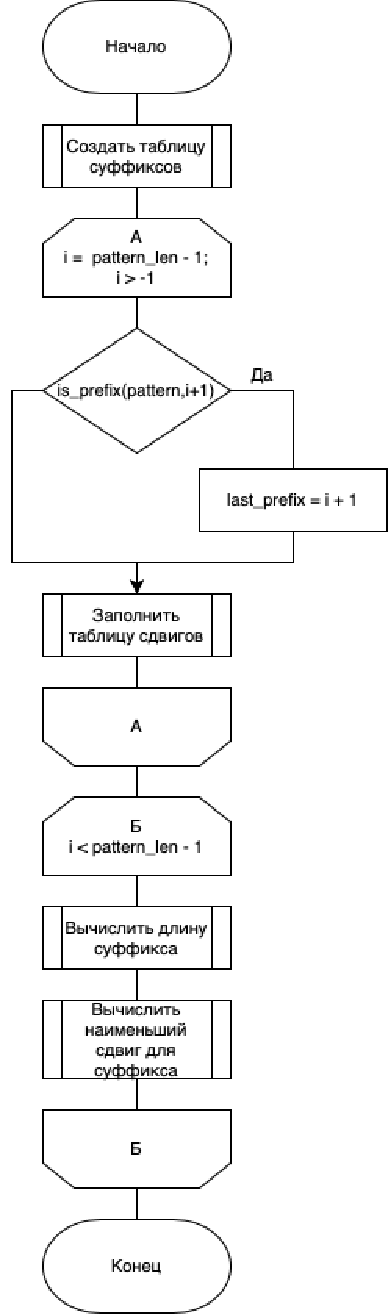
\includegraphics[width=0.4\linewidth]{img/bm4.pdf}
    \caption{Схема создания таблицы суффиксов}
    \label{img:bm4}
\end{figure}

\clearpage
\section{Псевдокоды рассматриваемых алгоритмов}
В листинге \ref{lst:std} представлен псевдокод стандартного алгоритма поиска подстроки в строке. 
В листингах \ref{lst:mur} -- \ref{lst:stop} показаны
псевдокоды алгоритма Бойера-Мура и дополнительных функций необходимых для поиска подстроки в строке.

\begin{lstlisting}[label=lst:std, caption = Псевдокод стандартного алгоритма поиска подстроки в строке]
i <- 0
result <- -1
text_len <- Длина строки
pattern_len <- Длина подстроки
До тех пор пока i <= text_len - pattern_len выполнять
    j <- 0

    До тех пор пока j < pattern_len и text[i + j] == pattern[j] выполнять
        j <- j + 1
    Конец цикла

    Если j == pattern_len тогда
        result <- i
        Выйти из цикла
    Конец условия

    i <- i + 1
Конец цикла

Возвратить result
\end{lstlisting}


\begin{lstlisting}[label=lst:mur, caption = Псевдокод функции поиска подстроки в строке в алгоритме Бойера-Мура]
text_len <- Длина строки
pattern_len <- Длина подстроки

bad_char_table <- Сгенерировать таблицу стоп символа
good_suffix_table <- Сгенерировать таблицу суффиксов

i <- pattern_len - 1

result <- -1
До тех пор пока i < text_len выполнять
    j <- pattern_len - 1

    До тех пор пока j >= 0 и text[i] == pattern[j] выполнять
        i <- i - 1
        j <- j - 1
    Конец цикла

    Если j == -1 тогда
        result <- i + 1
        Выйти из цикла
    Конец условия

    bad_char_shift <- Найти смещение в таблице стоп символа
    good_suffix_shift <- Найти смещение в таблице суффиксов

    i <-i + max(bad_char_shift, good_suffix_shift)
Конец цикла

Возвратить result
\end{lstlisting}

\begin{lstlisting}[label=lst:suff, caption = Псевдокод создания таблицы суффиксов]
pattern_len <- длина подстроки
suffix_table <- массив равный длине подстроки
last_prefix_position <- pattern_le

i <- pattern_len
До тех пор пока i > -1 выполнять
    Если подстрока является префиксом тогда
        last_prefix_position <- i + 1
    Конец условия
    suffix_table[pattern_len - 1 - i] <- last_prefix_position - i + pattern_len - 1
Конец цикла

i <- 0
До тех пока i < pattern_len - 1 выполнять
    j <- получить длину суффикса
    suffix_table[j] = min(suffix_table[j], pattern_len - 1 - i + j)

Возвратить suffix_table
\end{lstlisting}

\begin{lstlisting}[label=lst:stop, caption = Псевдокод создания таблицы стоп-символа]
bad_char_table <- создать словарь
pattern_len = <- длина подстроки

До тех пор пока i < pattern_len - 1 выполнять
    bad_char_table[pattern[i]] <- pattern_len - 1 - i

Возвратить bad_char_table
\end{lstlisting}

\section*{Вывод}

В данном разделе были разработаны алгоритм стандартного поиска подстроки в строке и алгоритм Бойера-Мура, также были 
выдвинуты требования к программному обеспечению.

